
\documentclass{exam}

\usepackage{units} 
\usepackage{graphicx}
\usepackage[fleqn]{amsmath}
\usepackage{cancel}
\usepackage{float}
\usepackage{mdwlist}
\usepackage{booktabs}
\usepackage{cancel}
\usepackage{polynom}
\usepackage{caption}
\usepackage{fullpage}
\usepackage{xfrac}
\usepackage{enumerate}

\newcommand{\degree}{\ensuremath{^\circ}} 
\everymath{\displaystyle}

% \begin{figure}[H]
%   \centering
%   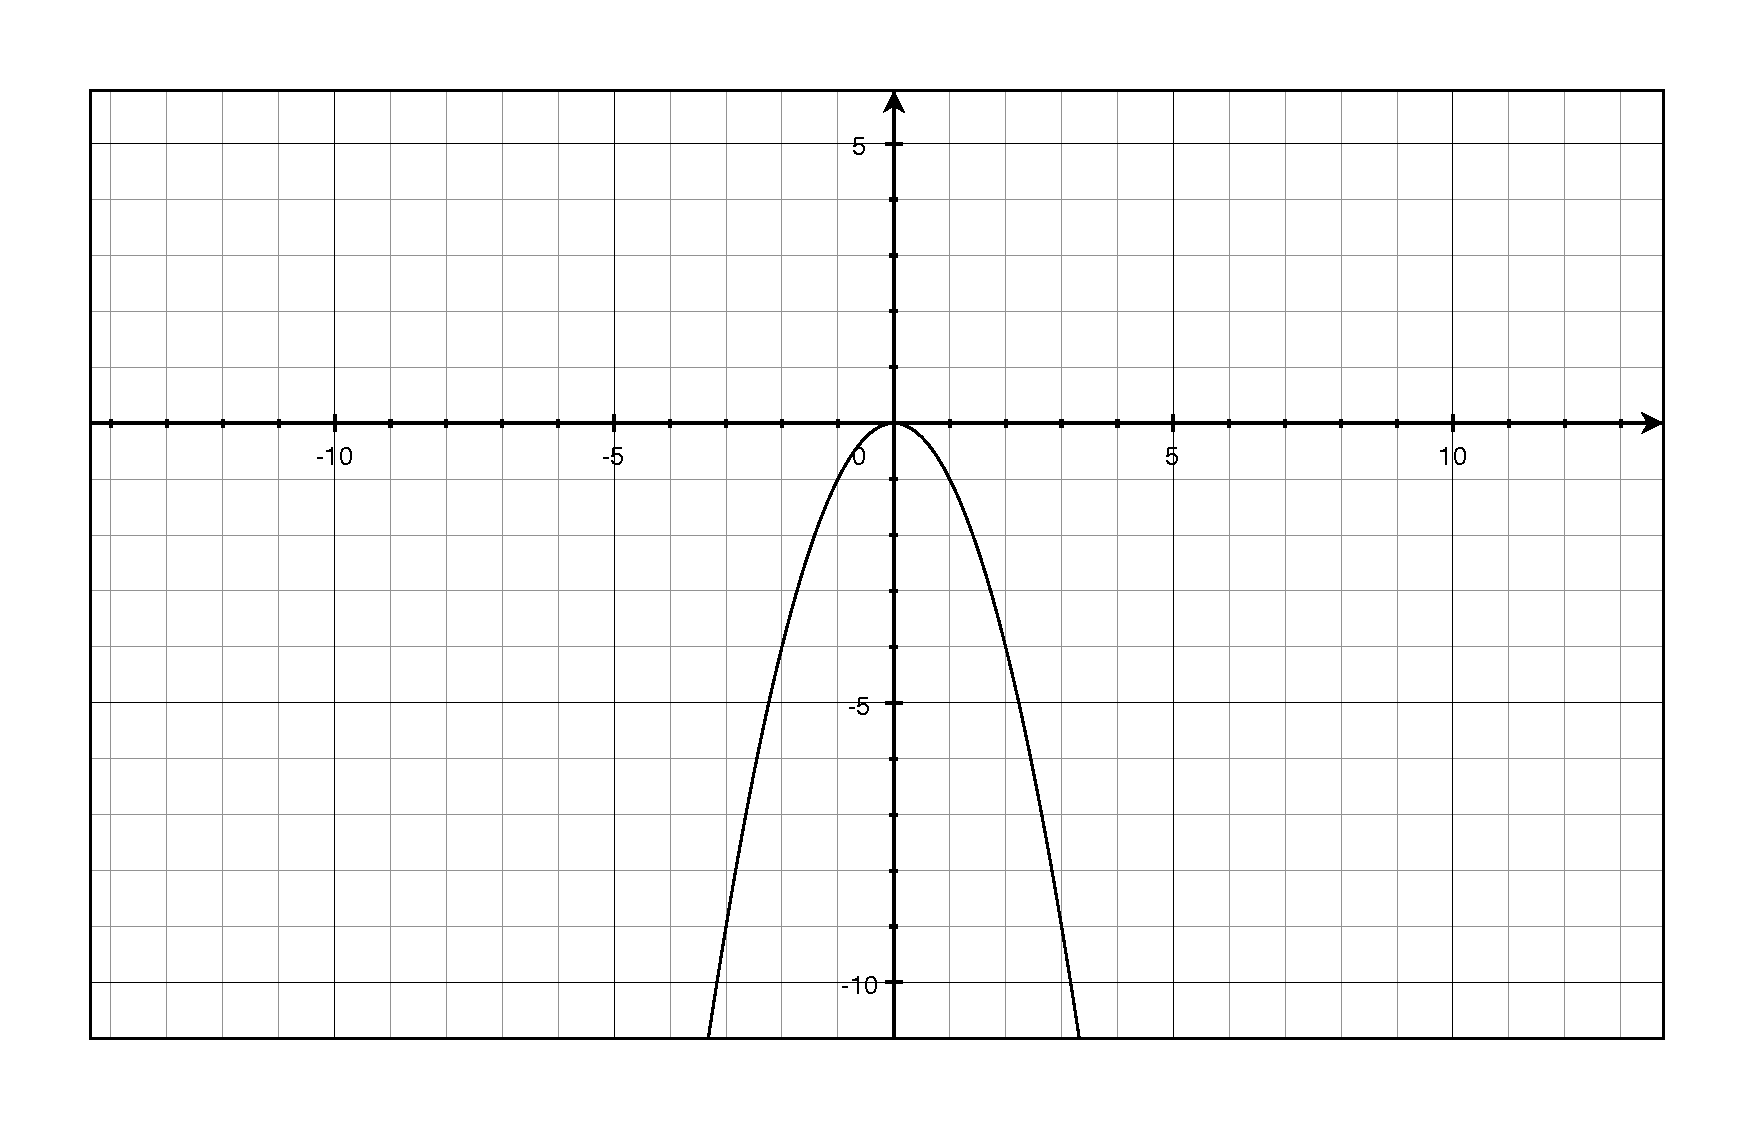
\includegraphics[scale=.3]{problem7.eps}
%   \caption*{Problem 7}
% \end{figure}

% \begin{tabular}{cc}
% \toprule
% period & amplitude \\
% \midrule
% value one & value two
% \bottomrule
% \end{tabular}

\printanswers

\ifprintanswers 
  \usepackage{2in1, lscape} 
\fi

\date{April 24, 2013}
\author{}
\title{Math 141 \\ Homework 10}

\begin{document}

\maketitle

\section{Homework}

\begin{itemize*}
  \item Read Section 3.4 
  \item Section 3.4: 1-27, 31-34, 38-66, 71-72, 77
\end{itemize*}

\section{Extra Credit}
Section 3.4: 80 and 81

\ifprintanswers
  \begin{description}
    \item[80]
      \begin{tabular}{lr}
        \toprule
        $n$         & $i^n$ \\
        \midrule
        $1$ & $i$ \\
        $2$ & $i^2 = -1$ \\
        $3$ & $i^3 = i^2 \cdot i = -i$ \\
        $4$ & $i^3 = (i^2)^2 (-1)^2 = 1$ \\
        \midrule
        $5$ & $i^5 = i^4 \cdot i   = i$ \\
        $6$ & $i^6 = i^4 \cdot i^2 = -1$ \\
        $7$ & $i^7 = i^4 \cdot i^3 = -i$ \\
        $8$ & $i^8 = i^4 \cdot i^4 = 1$ \\
        \midrule
        $9$  & $i^9    = i^8 \cdot i   = i$ \\
        $10$ & $i^{10} = i^8 \cdot i^2 = -1$ \\
        $11$ & $i^{11} = i^8 \cdot i^3 = -i$ \\
        $12$ & $i^{12} = i^8 \cdot i^4 = 1$ \\
        \bottomrule
      \end{tabular}

      Since the cycle repeats every four numbers, you can compute $i$ to any power by first finding the remainder of the
      power divided by four.  The remainder of 4,446 divided by 4 is 2, so:
      \[
        i^{4,446} = i^2 = \boxed{-1}
      \]
      
    \item[81]
      \begin{align*}
        (-1 + i \sqrt{3})^3 &= (-1 + i \sqrt{3})(-1 + i \sqrt{3})(-1 + i \sqrt{3}) \\
                           &= (-2 -2 i \sqrt{3})(-1 + i \sqrt{3}) \\
                           &= 8 \\
      \end{align*}

      \begin{align*}
        (-1 - i \sqrt{3})^3 &= (-1 - i \sqrt{3})(-1 - i \sqrt{3})(-1 - i \sqrt{3}) \\
                           &= (-2 + 2 i \sqrt{3})(-1 - i \sqrt{3}) \\
                           &= 8 \\
      \end{align*}

      The roots of $\sqrt[4]{16}$ are solutions to the equation $x^4 = 16$:
      \begin{align*}
        x^4                &= 16 \\
        x^4 - 16           &= 0 \\
        (x^2 - 4)(x^2 + 4) &= 0 \\
        \\
        x                  &= \boxed{\left\{ -2, 2, 2i, -2i \right\} } \\
      \end{align*}
  \end{description}

  \pagebreak

  \section{Section 3.4}

  \begin{description}
    \item[1] 
      \begin{tabular}{lr}
        \toprule
        number         & $5 - 7i$ \\
        \midrule
        real part      & $5$ \\
        \midrule
        imaginary part & $-7$ \\
        \midrule
        \bottomrule
      \end{tabular}

    \item[2] 
      \begin{tabular}{lr}
        \toprule
        number         & $-6 + 4i$ \\
        \midrule
        real part      & $-6$ \\
        \midrule
        imaginary part & $4$ \\
        \bottomrule
      \end{tabular}

    \item[3]
      \begin{tabular}{lr}
        \toprule
        number         & $\frac{-2 - 5i}{3}$ \\
        \midrule
        real part      & $- \frac{2}{3}$ \\
        \midrule
        imaginary part & $- \frac{5}{3}$ \\
        \bottomrule
      \end{tabular}

    \item[4]
      \begin{tabular}{lr}
        \toprule
        number         & $\frac{4 + 7i}{2}$ \\
        \midrule
        real part      & $2$ \\
        \midrule
        imaginary part & $\frac{7}{2}$ \\
        \bottomrule
      \end{tabular}

    \item[5]
      \begin{tabular}{lr}
        \toprule
        number         & $3$ \\
        \midrule
        real part      & $3$ \\
        \midrule
        imaginary part & $0$ \\
        \bottomrule
      \end{tabular}

    \item[6]
      \begin{tabular}{lr}
        \toprule
        number         & $- \frac{1}{2}$ \\
        \midrule
        real part      & $- \frac{1}{2}$ \\
        \midrule
        imaginary part & $0$ \\
        \bottomrule
      \end{tabular}

    \item[7]
      \begin{tabular}{lr}
        \toprule
        number         & $- \frac{2}{3} i$ \\
        \midrule
        real part      & $0$ \\
        \midrule
        imaginary part & $- \frac{2}{3}$ \\
        \bottomrule
      \end{tabular}

    \item[8]
      \begin{tabular}{lr}
        \toprule
        number         & $i \sqrt{3}$ \\
        \midrule
        real part      & $0$ \\
        \midrule
        imaginary part & $\sqrt{3}$ \\
        \bottomrule
      \end{tabular}

    \item[9]
      \begin{tabular}{lr}
        \toprule
        number         & $\sqrt{3} + \sqrt{-4} = \sqrt{3} + 2i$ \\
        \midrule
        real part      & $\sqrt{3}$ \\
        \midrule
        imaginary part & $2$ \\
        \bottomrule
      \end{tabular}

    \item[10]
      \begin{tabular}{lr}
        \toprule
        number         & $2 - \sqrt{-5} = 2 - i \sqrt{5}$ \\
        \midrule
        real part      & $2$ \\
        \midrule
        imaginary part & $-\sqrt{5}$ \\
        \bottomrule
      \end{tabular}

    \item[11] 
      \[
        (2 - 5i) + (3 + 4i) = \boxed{5 - i}
      \]

    \item[12] 
      \[
        (2 + 5i) + (4 - 6i) = \boxed{6 - i}
      \]

    \item[13] 
      \[
        (-6 + 6i) + (9 - i) = \boxed{3 + 5i}
      \]

    \item[14] 
      \[
        (3 - 2i) + \left( -5 - \frac{1}{3} i \right) = \boxed{-2 - \frac{7}{3} i}
      \]

    \item[15] 
      \[
        3i + (6 - 4i) = \boxed{6 - i}
      \]

    \item[16] 
      \[
        \left( \frac{1}{2} - \frac{1}{3} i \right) + \left( \frac{1}{2} + \frac{1}{3} i \right) = \boxed{1}
      \]

    \item[17] 
      \[
        \left( 7 - \frac{1}{2} i \right) - \left( 5 + \frac{3}{2} i \right) = \boxed{2 - 2i}
      \]

    \item[18] 
      \[
        (-4 + i) - (2 - 5i) = \boxed{-6 + 6i}
      \]

    \item[19] 
      \[
        (-12 + 8i) - (7 + 4i) = \boxed{-19 + 4i}
      \]

    \item[20] 
      \[
        6i - (4 - i) = \boxed{-4 + 7i}
      \]

    \item[21] 
      \[
        \frac{1}{3} i - \left( \frac{1}{4} - \frac{1}{6} i \right) = \boxed{- \frac{1}{4} + \frac{1}{2}i}
      \]

    \item[22] 
      \[
        (0.1 - 1.1 i) - (1.2 - 3.6 i) = \boxed{-1.1 + 2.5i}
      \]

    \item[23] 
      \[
        4(-1 + 2i) = \boxed{-4 + 8i}
      \]

    \item[24] 
      \[
        2i \left( \frac{1}{2} - i \right) = \boxed{2 + i}
      \]

    \item[25] 
      \[
        (7 - i)(4 + 2i) = 28 + 10i - 2i^2 = \boxed{30 + 10i}
      \]

    \item[26] 
      \[
        (5 - 3i)(1 + i) = 5 + 2i - 3i^2 = \boxed{8 + 2i}
      \]

    \item[27] 
      \[
        (3 - 4i)(5 - 12i) = 15 - 56i + 48i^2 = \boxed{-33 - 56i}
      \]

    \item[31] 
      \begin{align*}
        \frac{1}{i} &= \frac{1}{i} \cdot \left( \frac{i}{i} \right) \\
                    &= \boxed{-i} \\
      \end{align*}

    \item[32] 
      \begin{align*}
        \frac{1}{1 + i} &= \frac{1}{1 + i} \cdot \left( \frac{1 - i}{1 - i} \right) \\
                        &= \frac{1 - i}{1 - i^2} \\
                        &= \boxed{\frac{1}{2} - \frac{i}{2} } \\
      \end{align*}

    \item[33] 
      \begin{align*}
        \frac{2 - 3i}{1 - 2i} &= \frac{2 - 3i}{1 - 2i} \cdot \left( \frac{1 + 2i}{1 + 2i} \right) \\
                              &= \frac{2 + i - 6i^2}{1 - 4i^2} \\
                              &= \frac{8 + i}{5} \\
                              &= \boxed{\frac{8}{5} + \frac{i}{5} }
      \end{align*}

    \item[34] 
      \begin{align*}
        \frac{5 - i}{3 + 4i} &= \frac{5 - i}{3 + 4i} \cdot \left( \frac{3 - 4i}{3 - 4i} \right) \\
                             &= \frac{15 - 23i + 4i^2}{9 - 16i^2} \\
                             &= \frac{11 - 23i}{25} \\
                             &= \boxed{ \frac{11}{25} - \frac{23i}{25} } \\
      \end{align*}

    \item[38] 
      \begin{align*}
        (2 - 3i)^{-1} &= \frac{1}{2 - 3i} \cdot \left( \frac{2 + 3i}{2 + 3i} \right) \\
                      &= \frac{2 + 3i}{4 - 9i^2} \\
                      &= \frac{2 + 3i}{13} \\
                      &= \boxed{\frac{2}{13} + \frac{3i}{13}} \\
      \end{align*}

    \item[39] 
      \begin{align*}
        \frac{4 + 6i}{3i} &= \frac{4 + 6i}{3i} \cdot \left( \frac{i}{i} \right) \\
                          &= \frac{4i + 6i^2}{3i^2} \\
                          &= \frac{-6 + 4i}{-3} \\
                          &= \boxed{2 - \frac{4i}{3}} \\
      \end{align*}

      alternate solution:
      \begin{align*}
        \frac{4 + 6i}{3i} &= \frac{4}{3i} + \frac{6i}{3i} \\
                          &= 2 + \frac{4}{3i} \cdot \left( \frac{i}{i} \right) \\
                          &= \boxed{2 - \frac{4i}{3}} \\
      \end{align*}

    \item[40] 
      \begin{align*}
        \frac{-3 + 5i}{15i} &= \frac{1}{3} - \frac{1}{5i} \\
                            &= \frac{1}{3}  - \frac{1}{5i} \cdot \left( \frac{i}{i} \right) \\
                            &= \boxed{\frac{1}{3}  + \frac{i}{5}} \\
      \end{align*}

    \item[41] 
      \begin{align*}
        \frac{1}{1 + i} + \frac{1}{1 - i} &= \frac{1 - i - (1 + i)}{1 - i^2} \\
        &= \frac{-2i}{2} \\
        &= \boxed{-i} \\
      \end{align*}

    \item[42] 
      \begin{align*}
        \frac{(1 + 2i)(3 - i)}{2 + i} &= \frac{3 + 5i - 2i^2}{2 + i} \\
                                      &= \frac{5 + 5i}{2 + i} \left( \frac{2 - i}{2 - i} \right) \\
                                      &= \frac{10 + 5i - 5i^2}{4 - i^2}  \\
                                      &= \frac{15 + 5i}{5}  \\
                                      &= \boxed{3 + i} \\
      \end{align*}

    \item[43] 
      \[
        i^3 = i \cdot i^2 = \boxed{-i}
      \]

    \item[44] 
      \[
        (2i)^4 = 2^4 \cdot (i^2)^2 = \boxed{16}
      \]

    \item[45] 
      \[
        i^{100} = (i^2)^{50} = \boxed{1 }
      \]

    \item[46] 
      \[
        i^{1002} = i^2 \cdot (i^2)^{500} = \boxed{-1}
      \]

    \item[47] 
      \[
        \sqrt{-25} = \boxed{5i}
      \]

    \item[48] 
      \[
        \sqrt{\frac{-9}{4}} = \boxed{\frac{3}{2} i}
      \]

    \item[49] 
      \[
        \sqrt{-3} \sqrt{-12} = i \sqrt{3} \cdot 2i \sqrt{3} = 6 i^2 = \boxed{-6 }
      \]

    \item[50] 
      \[
        \sqrt{\frac{1}{3}} \cdot \sqrt{-27} = \frac{3 \sqrt{3}}{\sqrt{3}} i = \boxed{3i}
      \]

    \item[51] 
      \begin{align*}
        \left(3 - \sqrt{-5}\right)\left(1 + \sqrt{-1}\right) &= \left(3 - i \sqrt{5}\right)\left(1 + i\right) \\
                                       &= 3 + \left(3 - \sqrt{5}\right)i - i^2 \sqrt{5} \\
                                       &= \boxed{\left(3 + \sqrt{5}\right) + \left(3 - \sqrt{5}\right)i} \\
      \end{align*}

    \item[52] 
      \begin{align*}
        \frac{1 - \sqrt{-1}}{1 + \sqrt{-1}} &= \frac{1 - i}{1 + i} \left( \frac{1 + i}{1 + i} \right) \\
                                            &= \boxed{-i} \\
      \end{align*}

    \item[53] 
      \begin{align*}
        \frac{2 + \sqrt{-8}}{1 + \sqrt{-2}} &= \frac{2 + 2i \sqrt{2}}{1 + i\sqrt{2}} \left( \frac{1 - i\sqrt{2}}{1 - i\sqrt{2}} \right) \\
                                            &= \boxed{2} \\
      \end{align*}

    \item[54] 
      \begin{align*}
        \left( \sqrt{3} - \sqrt{-4} \right)\left( \sqrt{6} - \sqrt{-8} \right) 
           &= \left( \sqrt{3} - 2i \right)\left( \sqrt{6} - 2i \sqrt{2} \right) \\
           &= \boxed{-\sqrt{2}-4 i \sqrt{6}} \\
      \end{align*}

    \item[55] 
      \[
        \frac{\sqrt{-36}}{\sqrt{-2}\sqrt{-9}} = \frac{6i}{3i^2 \sqrt{2}} = - \frac{2i}{\sqrt{2}} = \boxed{- i \sqrt{2}}
      \]

    \item[56] 
      \[
        \frac{\sqrt{-7} \sqrt{-49}}{\sqrt{28}} = \frac{7i^2 \sqrt{7}}{2 \sqrt{7}} = \boxed{- \frac{7}{2}}
      \]

    \item[57] 
      \begin{align*}
        x^2 + 9 &= 0 \\
        \\
        x &= \frac{0 \pm \sqrt{0 - 4 \cdot 9}}{2} \\
          &= \boxed{\pm 3i} \\
      \end{align*}

    \item[58] 
      \begin{align*}
        9x^2 + 4 &= 0 \\
        \\
        x &= \frac{0 \pm \sqrt{0 - 4 \cdot 9 \cdot 4}}{2 \cdot 9} \\
        x &= \frac{\pm 12i}{18} \\
          &= \boxed{\pm \frac{2i}{3}} \\
      \end{align*}

    \item[59] 
      \begin{align*}
        x^2 - 4x + 5 &= 0 \\
        \\
        x &= \frac{4 \pm \sqrt{16 - 4 \cdot 5}}{2} \\
        x &= \frac{4 \pm 2i }{2} \\
          &= \boxed{2 \pm i} \\
      \end{align*}

    \item[60] 
      \begin{align*}
        x^2 + 2x + 2 &= 0 \\
        \\
        x &= \frac{-2 \pm \sqrt{4 - 4 \cdot 2}}{2} \\
        x &= \frac{-2 \pm 2i }{2} \\
        x &= \boxed{-1 \pm i} \\
      \end{align*}

    \item[61] 
      \begin{align*}
        x^2 + x + 1 &= 0 \\
        \\
        x &= \frac{-1 \pm \sqrt{1 - 4}}{2} \\
          &= \frac{-1 \pm i \sqrt{3}}{2} \\
          &= \boxed{-\frac{1}{2} \pm \frac{\sqrt{3}}{2} i} \\
      \end{align*}

    \item[62] 
      \begin{align*}
        x^2 - 3x + 3 &= 0 \\
        \\
        x &= \frac{3 \pm \sqrt{9 - 4 \cdot 3}}{2} \\
          &= \frac{3 \pm i \sqrt{3}}{2} \\
          &= \boxed{\frac{3}{2} \pm \frac{\sqrt{3}}{2} i} \\
      \end{align*}

    \item[63] 
      \begin{align*}
        2x^2 - 2x + 1 &= 0 \\
        \\
        x &= \frac{2 \pm \sqrt{4 - 4 \cdot 2}}{4} \\
          &= \frac{2 \pm 2i}{4} \\
          &= \boxed{\frac{1}{2} \pm \frac{1}{2} i} \\
      \end{align*}

    \item[64] 
      \begin{align*}
        2x^2 + 3      &= 2x \\
        2x^2 - 2x + 3 &= 0 \\
        \\
        x &= \frac{2 \pm \sqrt{4 - 4 \cdot 2 \cdot 3}}{4} \\
          &= \frac{2 \pm 2\sqrt{5} i}{4} \\
          &= \boxed{\frac{1}{2} \pm \frac{\sqrt{5}}{2} i} \\
      \end{align*}

    \item[65] 
      \begin{align*}
        t + 3 + \frac{3}{t} &= 0 \\
        t^2 + 3t + 3        &= 0 \\
        \\
        t &= \frac{-3 \pm \sqrt{9 - 4 \cdot 3}}{2} \\
          &= \frac{-3 \pm i \sqrt{3}}{2} \\
          &= \boxed{- \frac{3}{2} \pm \frac{\sqrt{3}}{2} i} \\
      \end{align*}

    \item[66] 
      \begin{align*}
        z + 4 + \frac{12}{z} &= 0 \\
        z^2 + 4z + 12        &= 0 \\
        \\
        z &= \frac{-4 \pm \sqrt{16 - 4 \cdot 12}}{2} \\
          &= \frac{-4 \pm 4 i \sqrt{2}}{2} \\
          &= \boxed{-2 \pm 2 i \sqrt{2}} \\
      \end{align*}

    \item[71]
      \begin{align*}
        \overline{z} + \overline{w} &= a_z - b_z i + a_w - b_w i \\
                                    &= (a_z + a_w) - (b_z + b_w) i \\
                                    &= \overline{z + w} \\
      \end{align*}

    \item[72]
      \begin{align*}
        z \cdot w &= (a_z + b_z i) (a_w + b_w i) \\
                  &= (a_z a_w) + (a_w b_z + b_w a_z) i + b_z b_w i^2 \\
                  &= (a_z a_w - b_z b_w) + (a_w b_z + b_w a_z) i \\
                                    \\
        \overline{z} \cdot \overline{w} &= (a_z - b_z i) (a_w - b_w i) \\
                                        &= a_z a_w - (a_w b_z + b_w a_z) i + b_z b_w i^2 \\
                                        &= (a_z a_w - b_z b_w) - (a_w b_z + b_w a_z) i \\
                                        &= \overline{z w} \\
      \end{align*}

    \item[77]
      \begin{align*}
        \overline{z} \cdot \overline{z} &= (a_z + b_z i) (a_z - b_z i) \\
                                        &= a_z^2 - b_z^2 i^2 \\
                                        &= a_z^2 + b_z^2 \\
      \end{align*}

  \end{description}

\else
  \vspace{10 cm}
  \begin{quote}
    \begin{em}
      Truth is ever to be found in simplicity, and not in the multiplicity and confusion of things.
    \end{em}
  \end{quote}

  \hspace{1 cm} --Isaac Newton


\fi

\end{document}

